\documentclass[12pt]{article}

\usepackage{sbc-template}
\usepackage{graphicx,url}
\usepackage[utf8]{inputenc}
\usepackage[brazil]{babel}

\sloppy

\title{Comparacao de Huffman e LZW na Compressao Lossless de Codigo-Fonte}

\author{Gabryel Boer\inst{1} \and Integrantes do Grupo\inst{1}}

\address{Universidade Federal do ABC (UFABC)\\
  Santo Andre -- SP -- Brazil
  \email{aluno@aluno.ufabc.edu.br}
}

\begin{document}

\maketitle

\begin{abstract}
  This work presents a computational application for lossless compression of source code files using Huffman and LZW algorithms. Experiments on Python and C files measure compression ratio, execution time, memory usage, and correlate results with Shannon entropy and lexical repetition profiles. Results show no absolute winner: Huffman performs better on small and high-entropy files with lower memory usage, while LZW achieves higher ratios on repetitive C code and decompresses faster on medium files.
\end{abstract}

\begin{resumo}
  Este trabalho apresenta uma aplicacao computacional de compressao lossless de arquivos de codigo-fonte usando os algoritmos de Huffman e LZW. Experimentos em arquivos Python e C medem taxa de compressao, tempo de execucao, uso de memoria e correlacionam resultados com entropia de Shannon e perfil de repeticao lexical. Os resultados mostram que nao ha vencedor absoluto: Huffman e superior em arquivos pequenos e de alta entropia com menor uso de memoria, enquanto LZW alcanca melhores taxas em codigo C repetitivo e descomprime mais rapido em arquivos medios.
\end{resumo}

\section{Introducao}

A compressao de dados lossless e essencial para reduzir custos de armazenamento e transferencia em repositorios de software, backups e pipelines de CI/CD. Dois algoritmos classicos, Huffman \cite{huffman1952} e LZW \cite{welch1984,ziv1977}, representam abordagens distintas: codificacao estatistica por frequencia de simbolos e compressao por dicionario adaptativo de padroes repetidos.

Este artigo compara Huffman e LZW aplicados a um estudo de caso realista: compressao de codigo-fonte (.py e .c). O objetivo e avaliar qual algoritmo e mais efetivo em complexidade de tempo, complexidade de espaco, tempo pratico de execucao e facilidade de implementacao. A contribuicao inedita consiste em um framework de benchmark que correlaciona perfil de redundancia lexical e entropia com o desempenho relativo dos algoritmos.

A Secao 2 apresenta o problema de pesquisa. A Secao 3 revisa trabalhos relacionados. A Secao 4 descreve a fundamentacao teorica. A Secao 5 detalha a aplicacao computacional. A Secao 6 analisa os resultados. A Secao 7 apresenta conclusoes e trabalhos futuros.

\section{Problema de Pesquisa}

O estudo de caso escolhido e a compressao lossless de codigo-fonte para armazenamento e versionamento de repositorios de software. Arquivos de codigo combinam dois perfis: distribuicao desigual de caracteres (espacos, chaves, keywords) e repeticao de tokens lexicais (\texttt{def}, \texttt{import}, \texttt{return}).

A justificativa pratica inclui reducao de espaco em backups, otimizacao de transferencia entre ambientes e analise comparativa de tecnicas classicas de compressao em dominio real. O benchmark utiliza quatro arquivos de codigo e um log como baseline de contraste.

\section{Trabalhos Relacionados}

Sayood \cite{sayood2017} apresenta fundamentos de compressao lossless incluindo Huffman e LZ. Nambiar et al. \cite{nambiar2025} comparam Huffman com LZW em payloads textuais de rede, observando trade-offs entre taxa e recursos. Shrividhiya et al. \cite{shrividhiya2021} propõem hibrido Huffman+LZW, distinto do escopo deste trabalho que compara os algoritmos individualmente.

O diferencial deste artigo e o foco em codigo-fonte com framework de correlacao perfil-desempenho, ausente nos trabalhos de referencia.

\section{Fundamentacao Teorica}

\subsection{Huffman}

Huffman constrói uma arvore binaria bottom-up combinando os dois menores pesos em uma fila de prioridade (min-heap). Simbolos frequentes recebem codigos curtos; simbolos raros recebem codigos longos. Complexidade: $O(n \log n)$ para construcao da arvore, $O(m)$ para codificacao, onde $n \leq 256$ e $m$ e o tamanho do arquivo. Requer transmissao da tabela de frequencias como metadado.

\subsection{LZW}

LZW inicializa dicionario com 256 simbolos e estende com subsequencias encontradas durante a leitura. Codificacao em passada unica com complexidade $O(m)$ amortizado via tabela hash. O dicionario e reconstruido na decodificacao sem metadados extras. Limite de 4096 entradas evita crescimento ilimitado.

\subsection{Comparacao Teorica}

Huffman explora frequencia estatistica; LZW explora repeticao de padroes. Em codigo-fonte, ambos os perfis coexistem, sugerindo resultados mistos conforme o arquivo.

\section{Aplicacao Computacional}

A aplicacao foi implementada em Python 3 com estruturas: \texttt{heapq} e arvore binaria (Huffman), \texttt{dict} (LZW), \texttt{BitWriter/BitReader} para fluxo de bits. O benchmark (\texttt{compare.py}) mede taxa, tempo, memoria (\texttt{tracemalloc}) e valida integridade via SHA-256.

O modulo \texttt{profile.py} calcula entropia de Shannon $H(x) = -\sum p(x_i) \log_2 p(x_i)$ e taxa de repeticao lexical de tokens Python/C. Repositório publico: \url{https://github.com/GabryelBoer/huffman-lzw-compression}.

\section{Analise dos Resultados}

A Tabela~\ref{tab:resultados} resume os experimentos. Em \texttt{requests\_sessions.py} (34 KB), Huffman alcancou taxa 1.73 e LZW 1.66; Huffman venceu em taxa, LZW em descompressao (14 ms vs 36 ms). Em \texttt{jansson\_dump.c}, LZW venceu em taxa (1.90 vs 1.73) com maior uso de memoria.

Arquivos pequenos (\texttt{encoder\_sample.py}, 1 KB) e de alta entropia (\texttt{high\_entropy\_payload.py}) favoreceram Huffman; LZW expandiu o arquivo (-33.6\% economia). O baseline \texttt{access.log} confirmou dominancia de LZW (taxa 6.76) em padroes altamente repetitivos.

\begin{table}[ht]
\centering
\caption{Resultados do benchmark em codigo-fonte}
\label{tab:resultados}
\begin{tabular}{|l|l|r|r|r|}
\hline
Arquivo & Algoritmo & Taxa & Economia (\%) & Memoria (KB) \\
\hline
requests\_sessions.py & Huffman & 1.73 & 42.1 & 110 \\
requests\_sessions.py & LZW & 1.66 & 39.7 & 871 \\
jansson\_dump.c & Huffman & 1.73 & 42.0 & 66 \\
jansson\_dump.c & LZW & 1.90 & 47.4 & 568 \\
encoder\_sample.py & Huffman & 1.19 & 15.9 & 20 \\
encoder\_sample.py & LZW & 0.98 & -1.6 & 99 \\
high\_entropy\_payload.py & Huffman & 1.28 & 22.1 & 64 \\
high\_entropy\_payload.py & LZW & 0.75 & -33.6 & 695 \\
\hline
\end{tabular}
\end{table}

A Figura~\ref{fig:ratio} ilustra taxas por arquivo. A correlacao perfil-desempenho confirma: alta entropia favorece Huffman; repeticao lexical moderada favorece LZW em C; arquivos pequenos penalizam LZW.

\begin{figure}[ht]
\centering
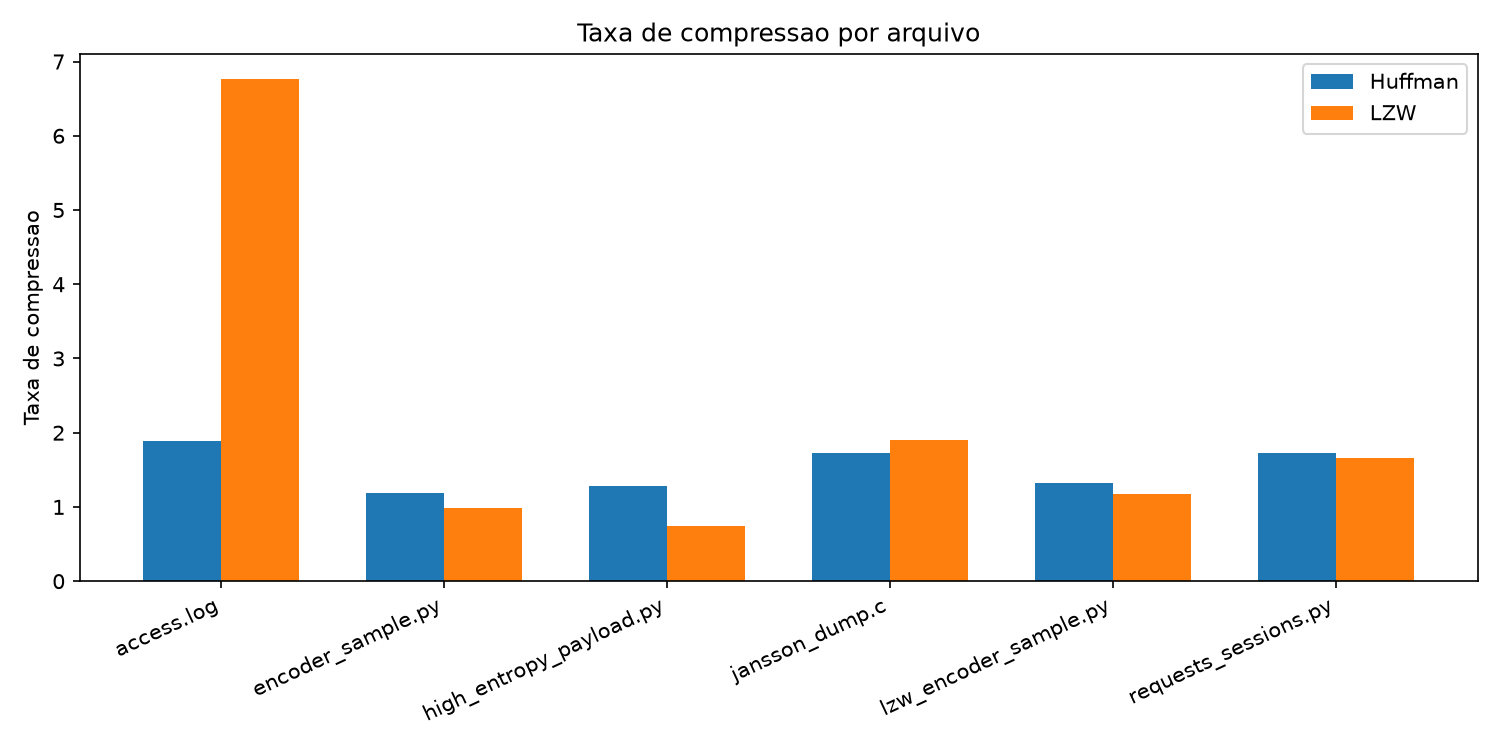
\includegraphics[width=.9\textwidth]{../benchmark-plots/compression-ratio.png}
\caption{Taxa de compressao por arquivo e algoritmo}
\label{fig:ratio}
\end{figure}

\textbf{Complexidade de tempo:} LZW tem vantagem teorica $O(m)$, mas Huffman foi competitivo na pratica. \textbf{Espaco:} Huffman usou 5--10x menos memoria. \textbf{Facilidade:} ambos sao moderados; Huffman exige heap e arvore; LZW exige tratamento de casos especiais na decodificacao.

\section{Conclusoes e Trabalhos Futuros}

Este artigo comparou Huffman e LZW na compressao lossless de codigo-fonte, com experimentos reproduziveis e analise de perfil de redundancia.

Nao ha vencedor absoluto. Huffman e mais efetivo em tempo de memoria e em arquivos pequenos ou de alta entropia. LZW e mais efetivo em taxa para codigo C repetitivo e em velocidade de descompressao em arquivos medios. A facilidade de implementacao e equivalente.

Trabalhos futuros incluem compressao de repositorios completos, integracao com Git, e avaliacao de variantes adaptativas e hibridas em escala de projetos reais.

\bibliographystyle{sbc}
\bibliography{referencias}

\end{document}
